%-------------------------
% Resume in Latex
% Author : Sourabh Bajaj
% License : MIT
%------------------------

\documentclass[letterpaper,11pt]{article}

\usepackage{graphicx}
\usepackage{latexsym}
\usepackage[empty]{fullpage}
\usepackage{titlesec}
\usepackage{marvosym}
\usepackage[usenames,dvipsnames]{color}
\usepackage{verbatim}
\usepackage{enumitem}
\usepackage[hidelinks]{hyperref}
\usepackage{fancyhdr}
\usepackage[english]{babel}
\usepackage{tabularx}

\pagestyle{fancy}
\fancyhf{} % clear all header and footer fields
\fancyfoot{}
\renewcommand{\headrulewidth}{0pt}
\renewcommand{\footrulewidth}{0pt}

% Adjust margins
\addtolength{\oddsidemargin}{-0.5in}
\addtolength{\evensidemargin}{-0.5in}
\addtolength{\textwidth}{1in}
\addtolength{\topmargin}{-.5in}
\addtolength{\textheight}{1.0in}

\urlstyle{same}

\raggedbottom
\raggedright
\setlength{\tabcolsep}{0in}

% Sections formatting
\titleformat{\section}{
  \vspace{-4pt}\scshape\raggedright\large
}{}{0em}{}[\color{black}\titlerule \vspace{-5pt}]

%-------------------------
% Custom commands
\newcommand{\resumeItem}[2]{
  \item\small{
    \textbf{#1}{: #2 \vspace{-2pt}}
  }
}

\newcommand{\resumeSubheading}[4]{
  \vspace{-1pt}\item
    \begin{tabular*}{0.97\textwidth}[t]{l@{\extracolsep{\fill}}r}
      \textbf{#1} & #2 \\
      \textit{\small#3} & \textit{\small #4} \\
    \end{tabular*}\vspace{-5pt}
}

\newcommand{\resumeSubItem}[2]{\resumeItem{#1}{#2}\vspace{-4pt}}

\renewcommand{\labelitemii}{$\circ$}

\newcommand{\resumeSubHeadingListStart}{\begin{itemize}[leftmargin=*]}
\newcommand{\resumeSubHeadingListEnd}{\end{itemize}}
\newcommand{\resumeItemListStart}{\begin{itemize}}
\newcommand{\resumeItemListEnd}{\end{itemize}\vspace{-5pt}}

%-------------------------------------------
%%%%%%  CV STARTS HERE  %%%%%%%%%%%%%%%%%%%%%%%%%%%%


\begin{document}

%----------HEADING-----------------
\begin{tabular*}{\textwidth}{l@{\extracolsep{\fill}}r}
  \textbf{\href{https://www.fosskers.ca/}{\Large Colin Woodbury}} & Email : \href{mailto:colin@fosskers.ca}{colin@fosskers.ca}\\
  \href{https://www.fosskers.ca/en/cv}{https://www.fosskers.ca/en/cv} & Mobile : +1-604-812-4532 \\
\end{tabular*}

\begin{figure}[h!]
  \centering
  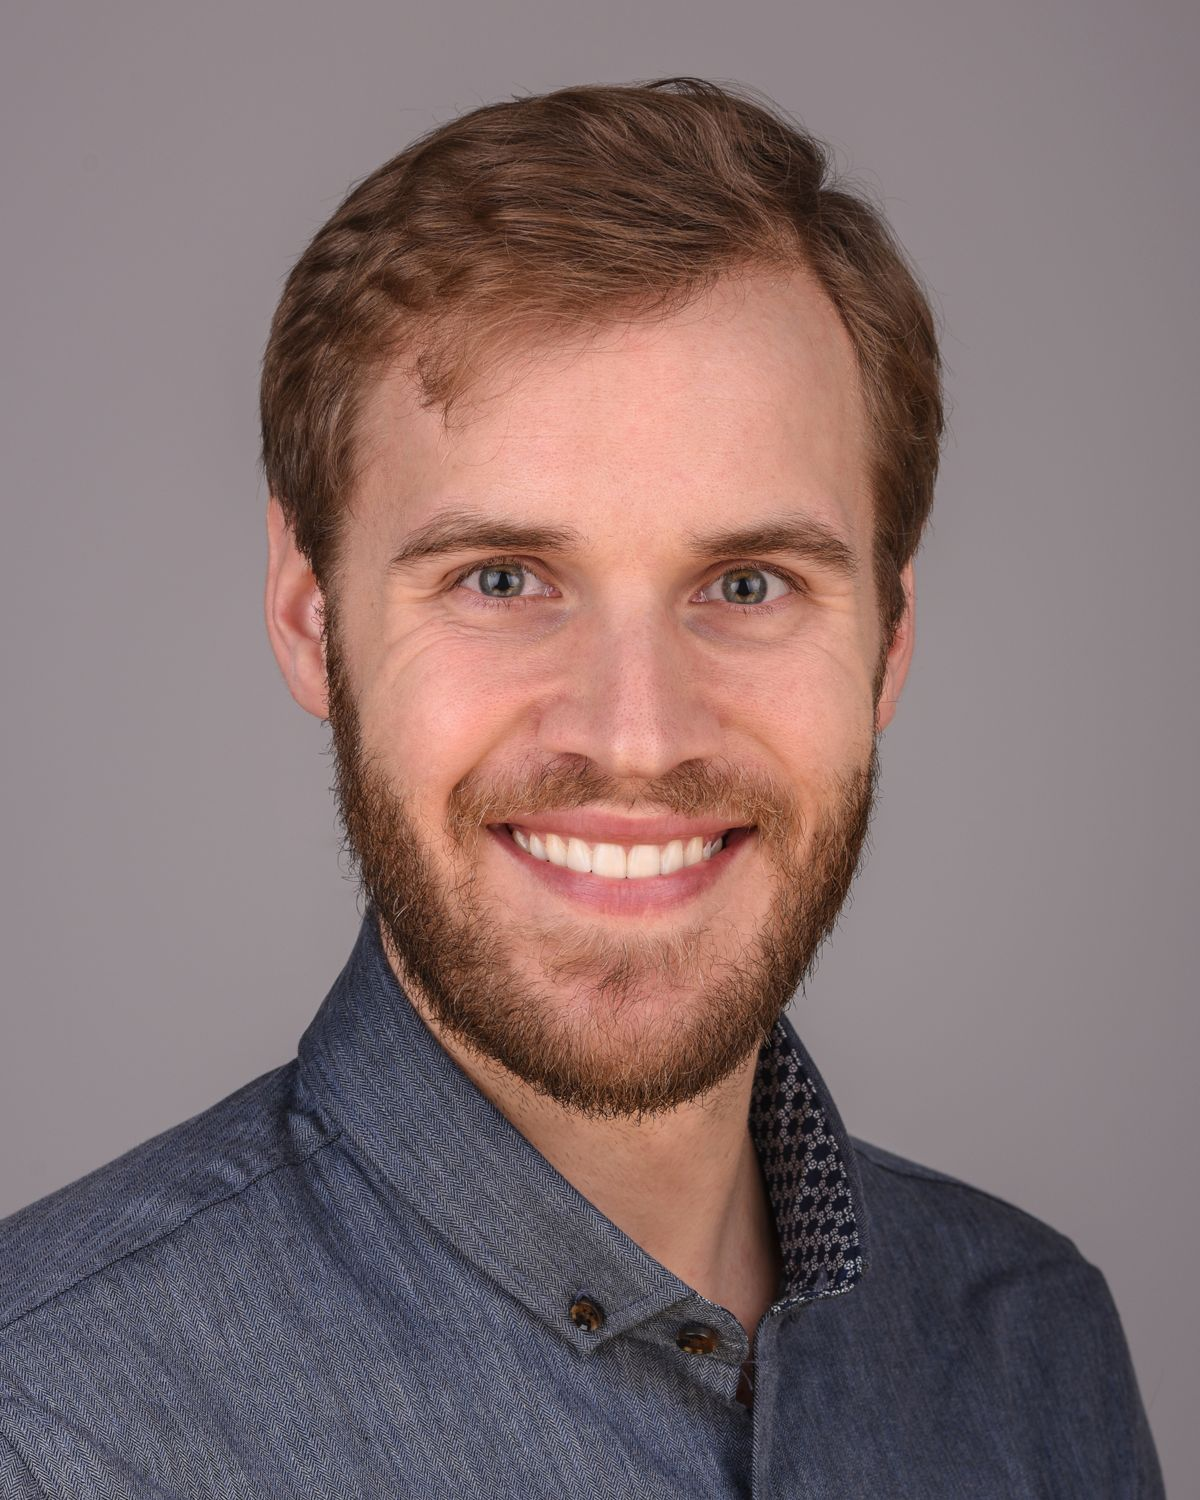
\includegraphics[width=0.25\linewidth]{colin.jpg}
\end{figure}

\begin{center}
  Full-stack developer and avid contributor to Open Source. \\
  Ranked Top 20 of Canadian Open Source Developers. \\
  Public speaker in both Japanese and English.
\end{center}

%--------PROGRAMMING SKILLS------------
\section{Skills}
\resumeSubHeadingListStart
\item{\textbf{Languages}{: Haskell, Rust, Go, Scala, Java, Python, C}}
\item{\textbf{Web Technologies}{: Terraform, GraphQL, AWS, Docker, Web Assembly}}
\item{\textbf{Other}{: Linux, Git, SQL, MongoDB, Apache Spark}}
\resumeSubHeadingListEnd

%-----------EXPERIENCE-----------------
\section{Experience}
\resumeSubHeadingListStart

\resumeSubheading
    {Kadena}{New York, USA}
    {Haskell Software Developer (Remote)}{2018 August - 2020 May}
    \resumeItemListStart
    \resumeItem{Backend Development}{Core developer of the Chainweb project, involving networking and algorithm design.}
    \resumeItem{System Administration}{Main sysadmin for Kadena web servers. Managed AWS servers with Terraform.}
    \resumeItem{Documentation}{Wrote extensive documentation in both Japanese and English.}
    \resumeItem{Public Speaking}{Represented the company as a speaker at conferences in Japan, the USA, and Canada.}
    \resumeItemListEnd

\resumeSubheading
    {Azavea}{Philadelphia, USA}
    {Scala Software Developer (Remote)}{2016 May - 2017 December}
    \resumeItemListStart
    \resumeItem{Backend Development}{Maintained GeoTrellis project, a library suite for batch processing of GIS data.}
    \resumeItem{Research}{Researched, designed, and implemented GIS algorithms and software.}
    %% \resumeItem{VectorPipe}{Wrote a library to process Vector Tile data through GeoTrellis.}
    %% \resumeItem{VectorTiles}{Wrote Haskell and Scala libraries that implement the Mapbox Vector Tiles spec.}
    \resumeItem{System Adminstration}{Managed production AWS servers with Docker and Terraform.}
    \resumeItemListEnd

\resumeSubheading
    {Adenda Media}{Vancouver, Canada}
    {Scala Software Developer}{2014 May - 2016 April}
    \resumeItemListStart
    \resumeItem{Backend Development}{Maintained and enhanced a Play + MySQL backend.}
    \resumeItem{Frontend Development}{Implemented a Twitter Bootstrap-based web application.}
    \resumeItem{Artificial Intelligence}{Implemented a content recommendation system using Apache Spark's MLlib.}
    \resumeItemListEnd

\resumeSubheading
    {Sasebo Board of Education}{Sasebo, Japan}
    {English Teacher (ALT)}{2010 August - 2013 July}
    \resumeItemListStart
    \resumeItem{English Teaching}{Taught English to Elementary and Middle School students. Supported Japanese colleagues.}
    \resumeItem{English Club}{Ran an English Club and coached students to participate in English speech contests.}
    \resumeItemListEnd

\resumeSubHeadingListEnd

%-----------EDUCATION-----------------
\section{Education}
\resumeSubHeadingListStart
\resumeSubheading
    {Simon Fraser University}{Vancouver, Canada}
    {Post-Baccalaureate Diploma in Computing Science}{2013 September - 2016 April}
    \resumeItemListStart
    \resumeItem{Student Council}{2014: CSSS Vice President. 2015: CSSS President.}
    \resumeItem{SFU Choir}{President}
    \resumeItem{Honour Roll}{Made the Dean's Honour Roll two years in a row.}
    \resumeItemListEnd

\resumeSubheading
    {Saga University}{Saga, Japan}
    {SPACE Exchange Program for International Students}{2008 September - 2009 August}
    \resumeItemListStart
    \resumeItem{Club Activities}{Member of the Tea Ceremony Club.}
    \resumeItem{Public Speaking}{Winner of the year-end Speech Contest.}
    \resumeItemListEnd

\resumeSubheading
    {University of Manitoba}{Winnipeg, Canada}
    {Bachelor of Arts in Asian Studies}{2006 September - 2010 April}
    \resumeItemListStart
    \resumeItem{Area of Study}{Major: Asian Languages and History. Minor: Computer Science.}
    \resumeItem{Honour Roll}{Made the Dean's Honour Roll.}
    \resumeItemListEnd

\resumeSubHeadingListEnd

%-----------CERTIFICATIONS-----------
\section{Certifications}
\resumeSubHeadingListStart
\resumeSubItem{Japanese Language Proficiency (JLPT)}{N1}
\resumeSubItem{Japanese Kanji Proficiency}{Level Pre-2}
\resumeSubHeadingListEnd

%-----------PROJECTS-----------------
\section{Open Source Projects}
\resumeSubHeadingListStart
\resumeSubItem{\href{https://github.com/aurapm/aura}{Aura}}{(Haskell) Package manager for Arch Linux.}
\resumeSubItem{\href{https://github.com/fosskers/active}{Active}}{(Go) Tool for keeping Github Actions up to date.}
\resumeSubItem{\href{https://github.com/fosskers/credit}{Credit}}{(Rust) Tool for measuring Github repository statistics.}
\resumeSubItem{\href{https://github.com/fosskers/rs-kanji}{Kanji}}{(Rust) Library for analysis of Japanese Kanji.}
\resumeSubItem{\href{https://github.com/fosskers/mapalgebra}{MapAlgebra}}{(Haskell) Library for efficient, polymorphic Map Algebra.}
\resumeSubItem{\href{https://github.com/geotrellis/vectorpipe}{VectorPipe}}{(Scala) VectorTile processing via GeoTrellis.}
\resumeSubHeadingListEnd

%-----------HOBBIES-----------
\section{Hobbies}
\resumeSubHeadingListStart
\resumeSubItem{Open Source Development}{Aura and library maintenance.}
\resumeSubItem{Rock Climbing}{Top Rope and Bouldering.}
\resumeSubItem{Language Study}{Japanese, German, Italian, and Esperanto.}
\resumeSubItem{Music}{Choirs and Saxophone.}
\resumeSubHeadingListEnd

\end{document}
